\documentclass[uplatex,dvipdfmx]{jsarticle}

\usepackage[uplatex,deluxe]{otf} % UTF
\usepackage[noalphabet]{pxchfon} % must be after otf package
\usepackage{stix2} %欧文&数式フォント
\usepackage[fleqn,tbtags]{mathtools} % 数式関連 (w/ amsmath)
\usepackage{hira-stix} % ヒラギノフォント&STIX2 フォント代替定義(Warning回避)


\usepackage{ascmac}
\usepackage{url}
\usepackage{float}
\usepackage{moreverb}
\usepackage{lscape}

\begin{document}

\title{自転車姿勢制御モジュールの提案}
\author{25G1065 塩澤匠生}
\date{2025年6月11日}
\maketitle
\section{はじめに}

社会的背景として自転車の単独事故は年5497件発生していて,その割合は年々増加している
というものがある\cite{jikokensuu}.

そして,
単独事故の原因の内7割が転倒事故であるというものがある\cite{tandokuWariai}.

\subsection{問題点}

ここで,自動車の単独事故の原因の内訳と比較してみると,車の単独事故における転倒(横転)事故の割合は1\%
である一方で,自転車の転倒事故の原因の内7割が転倒事故であることから自転車は乗り物の性質上転倒事故が発生しやすいという問題があると考えることができる.

%一般的な社会的背景を記述したパラグラフを複数配置, パラグラフの終わりは\parを入れる。
%最終パラグラフにはアイデアを記述する.

\subsection{目的}
問題を解決することにより,自転車で転倒事故が発生しない,または発生しにくくすることで
自転車の転倒事故を減少させることを目的とする.

\subsection{主張}

現状,自転車は乗り物の性質上転倒事故が発生するという問題に対して走行中に自転車の転倒を抑制するという製品はない.
そのため今は自転車の転倒事故を減少させるためには呼びかけなどの活動が行われている.

しかし,呼びかけによって乗り手の注意力を高めたとしても急な転倒や
路面状況による転倒など意識するだけでは防ぐことのできない転倒事故がある.

そこで我々は
自転車姿勢制御モジュールというものを提案する.
外付けで物理的に転倒を抑制するモジュールを
提案するこで呼びかけによって転倒に対して
乗り手に注意を促すよりも確実に転倒事故を防止,減少させられることに対する
アプローチになると考えられる.
\section{解決策としての提案手法}

自転車の性質上,転倒事故が発生しやすいという問題に対して我々は自転車姿勢制御モジュールというものを
提案する.自転車姿勢制御モジュールの概念図を図\ref{fig:moduleGainenn}に示す

\begin{figure}[H]
    \centering
    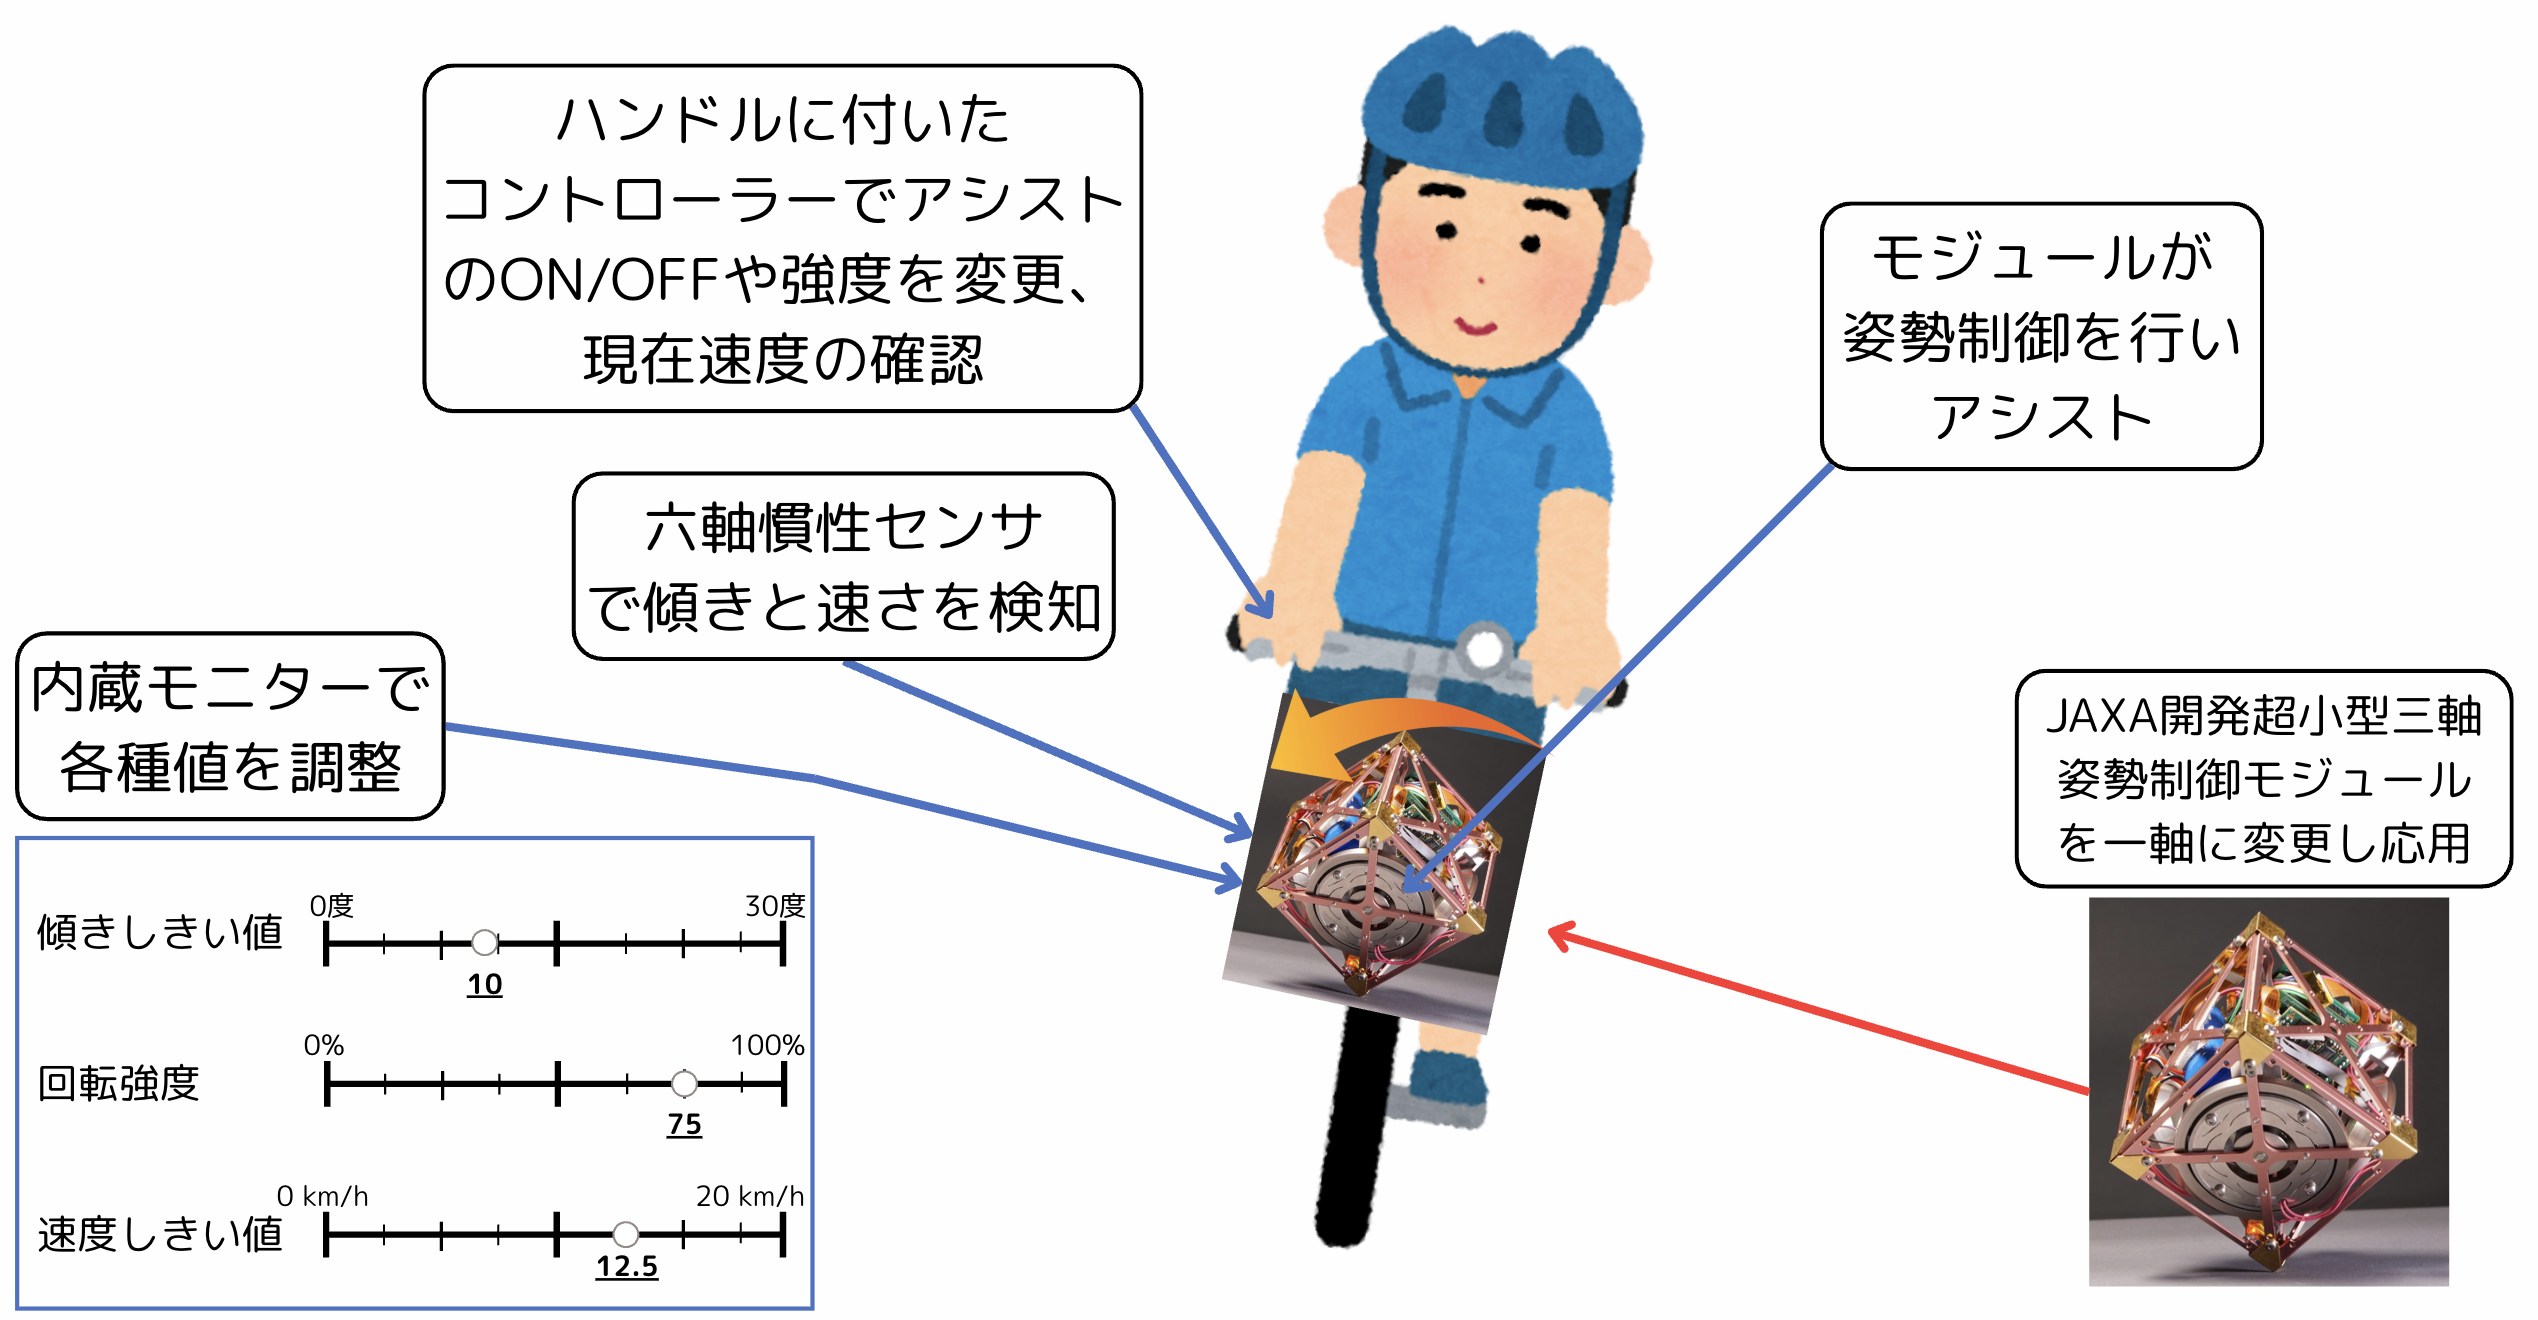
\includegraphics[width=0.8\textwidth]{fig/moduleGainenn2.png}
    \caption{自転車姿勢制御モジュールの概念図}
    \label{fig:moduleGainenn}
\end{figure}

まず,先行研究として,JAXAが開発した超小型三軸姿勢制御モジュールに付いての解説を行う.\cite{jaxaModule}
このモジュールは人工衛星の小型化を図るために作られたもので,慣性センサから本体の傾きを検知し,
ブラシレスDCモータでフライホイールを回転させることで生まれた力を用いて本体の姿勢を制御するものである.
サイズは$10×10×10 {cm}^3$である.

次に,提案するモジュールに付いての解説を行う.提案する自転車姿勢制御モジュールは先行研究で用いられている技術を応用し,
姿勢制御を行う軸を三軸から一軸に変更することで小型化と軽量化を図り,自転車に搭載しやすくしたモジュールである.
このモジュールは搭載されている六軸慣性センサーにより自転車の傾き,自転車の速度,横方向加速度を取得し,
取得した情報を下にモーターを回転させ,モーターの回転によって生まれる力で自転車の姿勢を保つものである.
また,自転車のハンドル部分にコントローラーを取り付けることで,アシストのON/OFFやアシストの強度変更を運転中に行うことができる
様になっている.このコントローラーには速度のモニターもついており,走行速度の確認も同時に行えるように
なっている.

このモジュールが動作する条件は,低速時に車体のふらつきを検知したとき,急な転倒を検知したとき,
コントローラーからの操作でアシストONが指定されたときの3つである.
低速時に車体のふらつきを検知したときの制御に関しては,アシスト自動OFF速度の設定を行うことにより,
自転車が設定した速度以上に達し,十分車体が安定したと判断される場合は自動でふらつきを検知したときの制御がOFF
になり,車体を傾けてのカーブが可能になる.
急な転倒を検知したときの制御に関しては六軸慣性センサーで車体の横方向の加速度の急激な変化を検知し,
転倒を検知したときに強力なアシストを行う機能である.

検出される傾きのしきい値やモーターの回転力の強さ,アシスト自動OFF速度のしきい値など,
乗る人によって個別に設定が必要な項目についてはモジュールに取り付けられたモニターで細く設定することができる.
自転車後輪上部にある荷台への取り付けを可能にすることで様々な自転車に特別な取り付け器具無しでつけられる様に
することを想定している.

次にモジュールの制御に関する具体的な流れ図を図\ref{fig:nagare}に示す.
\begin{figure}[H]
    \centering
    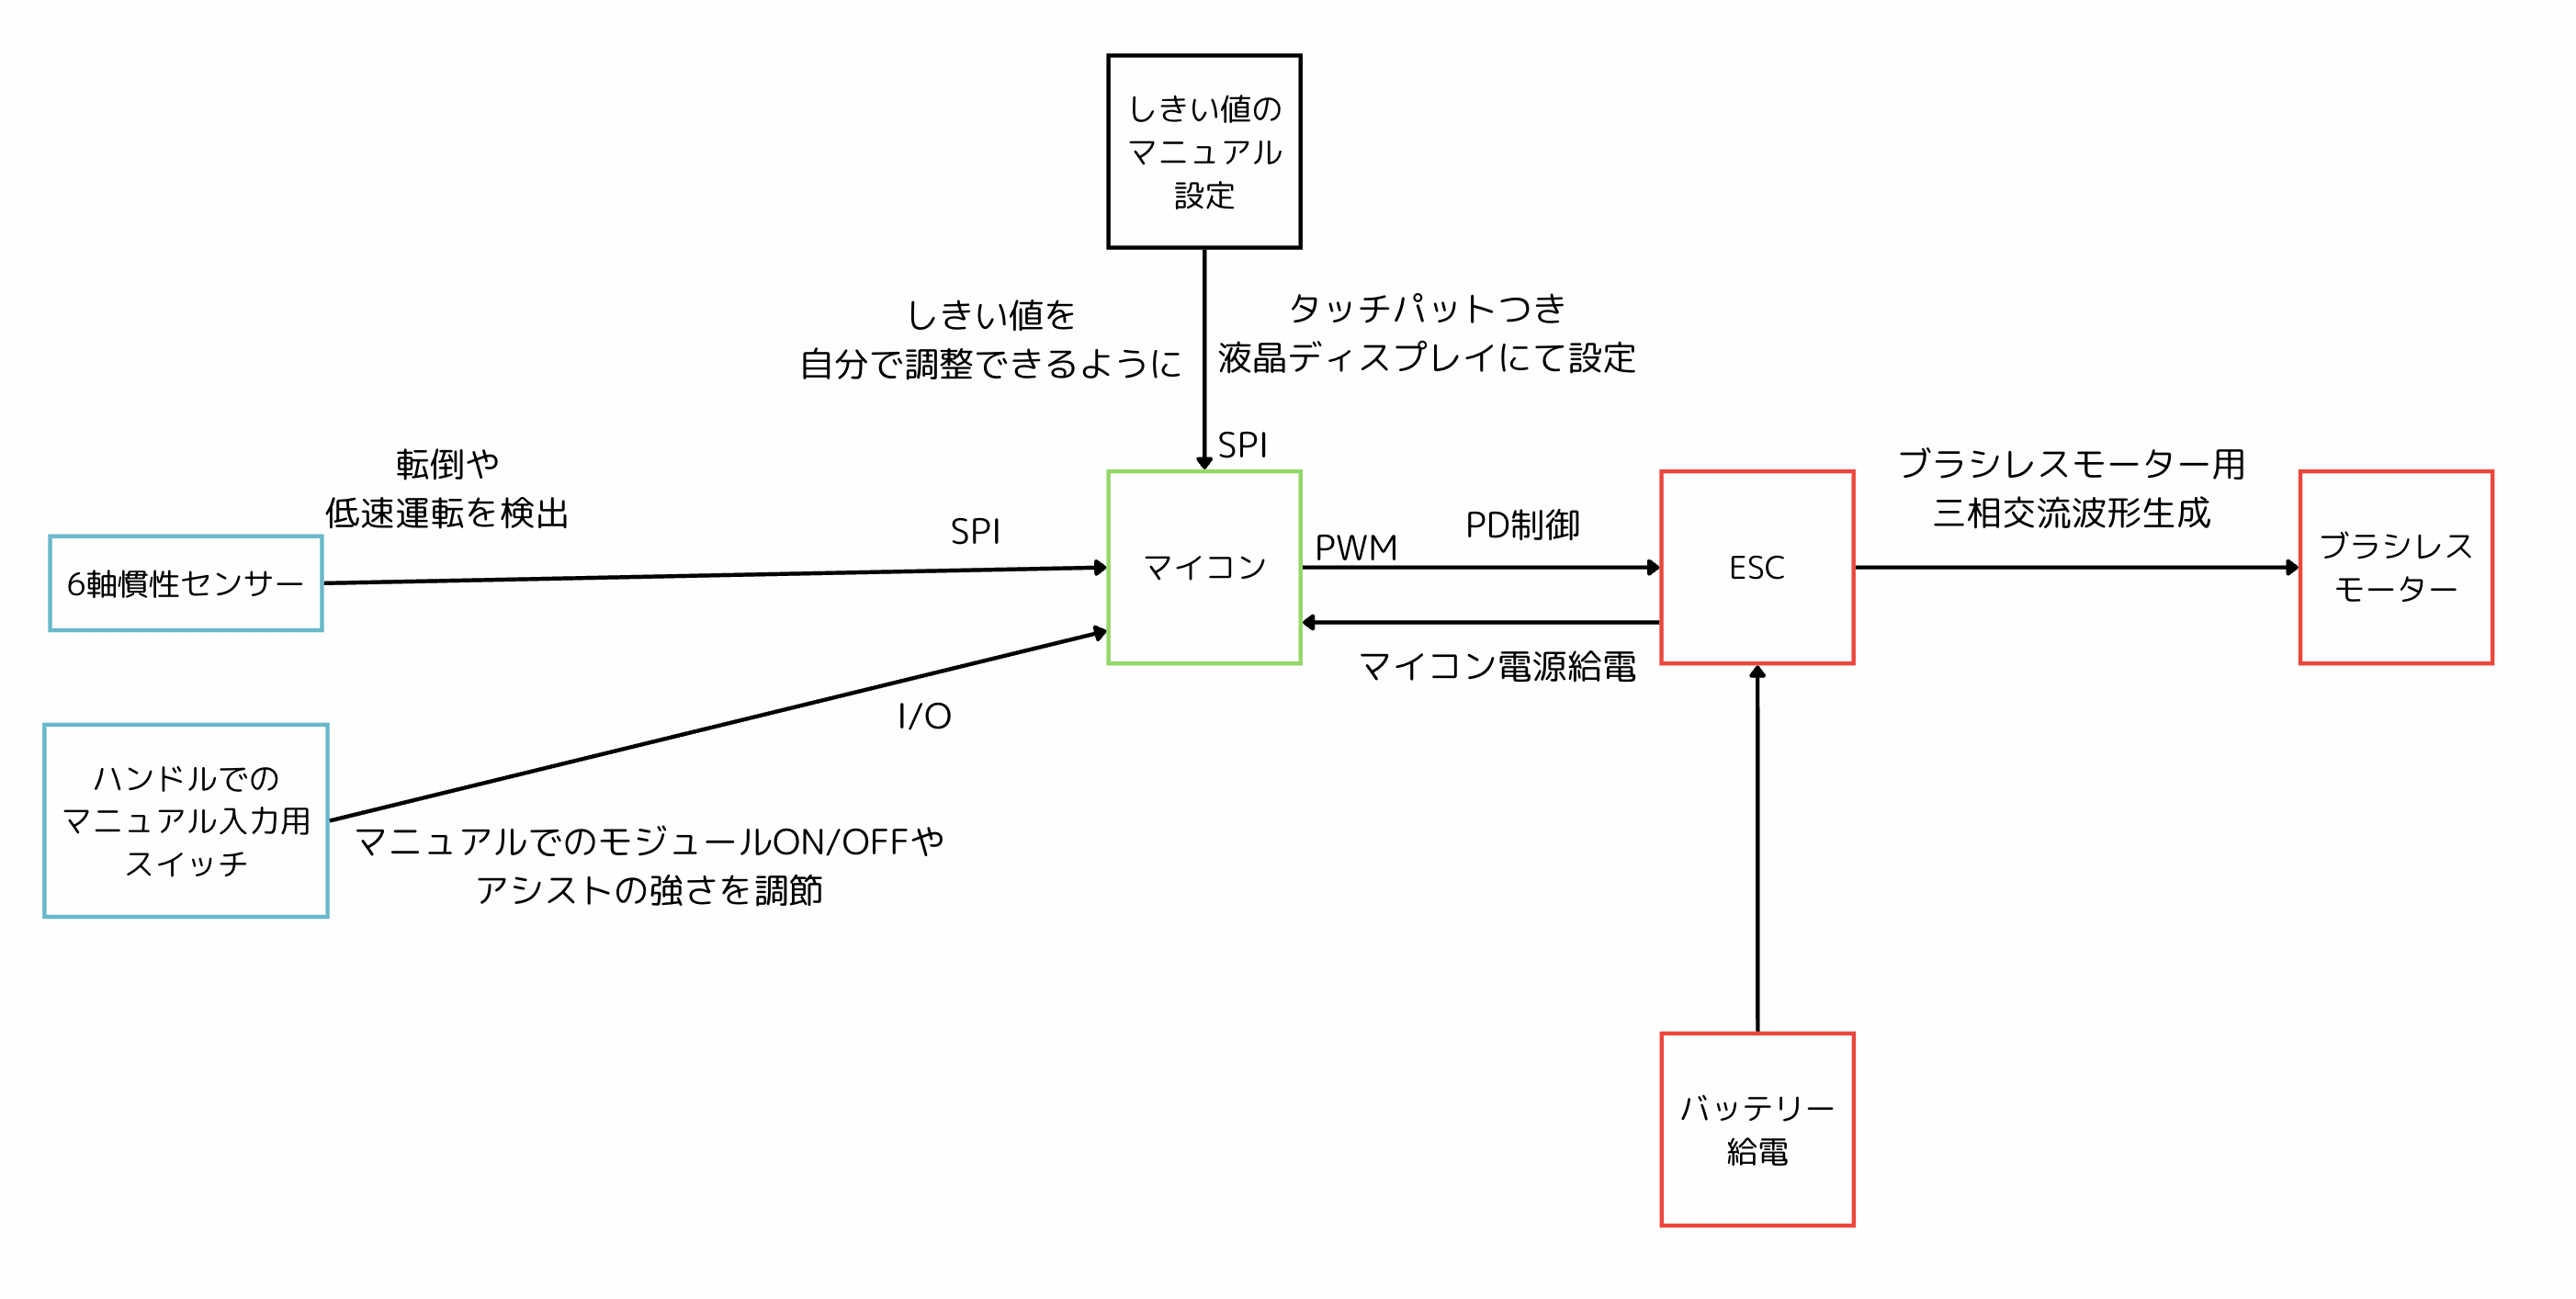
\includegraphics[width=0.8\textwidth]{fig/nagare.png}
    \caption{自転車姿勢制御モジュールの制御の流れ図}
    \label{fig:nagare}
\end{figure}

制御用マイコンへの入力として,6軸慣性センサー,ハンドル部のコントローラーがあり,そのデータ基づいて
マイコンがPID制御を行い,適切なPWM波形を生成し,ESCに対して出力.そしてESCがPWM波形を三相交流電圧
に変換し,ブラシレスモーターを制御するという流れになっている.ここでESCに付いての解説を行う.ブラシレスモーターはDCモーター
と違い,制御するために単純な直流電圧ではなく三相交流電圧が要求される.そこで,PWM波形に基づいて
三相交流波形を生成するものがESCである.

そして次にモジュールを実現するための部品の選定を行ったところ,

\section{提案手法の実現可能性の評価と妥当性の検証}



\subsection{モジュールに対しての要件を満たすような素子,モーターがあるかについての考察}\label{subsec:youken}


次に提案するモジュールに対しての要件を満たすような素子,モーターがあるかについての考察を行う.

まず,6軸慣性センサについて考える.今回6軸慣性センサには車体の速度検出,車体の傾き検出,そして
急な転倒の検知が求められる.そこでデータの取得が高速かつデータの精度の高いセンサーが要求される.
そこで今回はPanasonicが販売しているEWTS5Gを使用するのが適切だと考えられる.
EWTS5Gはマイコンとの通信方式が$SPI$であり,他のシリアルの規格である$I^2c$や$UART$
と比べて高速なデータ通信が可能であり,感度出力誤差も$\leq \pm 3.0\%$であることから精度も
申し分ないと考えられるので,自転車姿勢制御モジュールの6軸慣性センサとして適していると考えられる.


自転車の姿勢を保てるほどの強力なモーターに関してはブラシレスモーターを使用するのが適切と考えられる.
ブラシレスモーターはDCモーターに比べ小型でも強い力を生み出すことができるのでこのモジュール
の要件に適している.実験を行ったわけではないのでどのくらいのパワーがあれば
自転車の姿勢制御が十分に行えるかはわからないが,今回はネットで売られている商品の内
なるべく1ボルトあたりの無負荷回転数が高いものを使用する想定にする.無負荷回転数が高ければ,
フライホイールを高速で回し,大きな力を得ることが可能だと考えられる.また,1ボルトあたりの無負荷回転数
が増えるとモーターのトルクが下げるという問題があるが,もしフライホイールを回すためのトルクが足りなかった場合は
減速ギアを使用し,トルクを上げることで対応可能である.
そして,もう一つのブラシレスモーターの選定基準として,センサー付きかという基準を設ける.
ブラシレスモーターにはセンサー付きのものがあり,このセンサー付きのモデルは
ローターの位置を把握する事ができ,これにより,スムーズなモーターの始動制御が可能になる.
自転車姿勢制御モジュールは細かな制御が必要だと考えられるため,このセンサーがついていることは
必須の条件だと考えられる.
これらの基準から部品の選定を行うと1ボルトあたりの無負荷回転数が4150回転と高く,
センサー付きのブラシレスモーターである
ジーフォース社のNeo Fast 8.5Tというモーターを
使用するのが適切であると考えられる.


次にNeo Fast 8.5Tも動かすことができるESCの選定をする.
Neo Fast 8.5Tは
対応電圧$8.4V$,最大出力$345W$なので電流量$I=W/V$で求めると$I=41A$となり,ESC
の出力できる電流量が$41A$以上のものを搭載しなければならない.また,モーター
始動時の突入電流のことを考慮し選定を行ったところ,
ジーフォース社のBLC50 Type-Dを使用するのが適切だと考えられる.このESCは
連続最大電流が$50A$でブラシレスモーターの電流に耐えることができ,また,瞬間最大電流
が$300A$なので突入電流に対しても十分強いことが考えられる.

次にバッテリーに付いて考える.BLC50 Type-Dは$2$セル$7.4V$のリポバッテリーか
4-6セル$4.8〜7.2V$のニッケル水素電池に対応している.
今回はニッケル水素電池に比べて小型でも充電容量が多く,高い電流を流すことのできる
$2$セル$7.4V$のリポバッテリーを使用するものとする.
条件にあう商品を調べたところ,容量も十分なSIGP 2S 7.4Vリチウム電池 6000mAh
という商品が見つかったのでこの商品を使用する想定とする.

マイコンは$SPI$での通信とPWM出力ができるものが要求される.
この条件は昨今のマイコンにはだいたい当てはまるので今回は
なるべく開発しやすく安価で高性能なマイコンを選ぶ.
この条件で考えた場合Espressif Systems社の販売しているESP32-DevKitC
を使用するのが望ましい.このマイコンは一枚1,384円と安価かつ
arduinoやPlatformIOといった統合開発環境での開発が可能なので
使用するのに適していると考えられる.

次にしきい値等の調整に用いる液晶モジュールについて考える.


これらのことから,このモジュールの要件を満たすような素子,モーターは実在
する事がわかるので制作が可能だと考えられる.

\subsection{コストに関する考察}

次にコスト面に付いての考察を行う.
まずは,\ref{subsec:youken}
で取り上げた製品の値段をまとめる.まとめた結果を表\ref{table:Price}に示す.

\begin{table}[h]
  \centering
  \caption{\ref{subsec:youken}で取り上げた製品の値段表}
  \label{table:Price}
  \begin{tabular}{|c|l|r|}
\hline
項目番号 & 製品名 & 値段(円) \\\hline \hline
1 & 6軸慣性センサー(Panasonic EWTS5G) & 2,974 \\\hline
2 & ブラシレスモーター(Neo Fast 8.5T) & 7,800 \\\hline
3 & ESC(BLC50 Type-D) & 7,700 \\\hline
4 & リポバッテリー(SIGP 2S 7.4V 6000mAh) & 4,199 \\\hline
  \end{tabular}
\end{table}

急な転倒にはどのような対応をするか

どのような場面でアシストをONにするか(車体を傾けて曲がりたいのに傾けられなくなってしまうのではないか)

アシストのしきい値や強さの変更をすることができるか

既存のジャイロスコープを取り付けた自転車の安定化モジュールとの違い

提案するうえでの課題(モーターの出力が足りるか検証できていない)

\section{おわりに}
%全体のまとめを簡潔に記述して,結論を述べる.

転倒防止できて問題点に対する対処ができているか

背景に対してどのような効果を発揮することが望めるか




\begin{thebibliography}{9}

\bibitem{jikokensuu} NEONAVI, 【自転車事故の実態】を知って安全に利用しよう~令和5年「交通事故統計」から, 
2025年6月11日閲覧,\url{https://neonavi.info/11203/}

\bibitem{tandokuWariai} 東京海上日動, 便利な自転車は運転次第で危険な乗り物になる, 
2025年6月11日閲覧,\url{https://www.tokiomarine-nichido.co.jp/world/guide/drive/202105.html}

\bibitem{jaxaModule} 礒川悌次郎, \& 信川創. (2023). 脳・神経系における機能創発の解明を目指した数理モデリングとデータ駆動分析―局所神経回路から大域的全脳レベルまで―. 計測と制御, 62(10), 587-592.

\end{thebibliography}

\end{document} 
